% 
% Licensed to the Apache Software Foundation (ASF) under one
% or more contributor license agreements.  See the NOTICE file
% distributed with this work for additional information
% regarding copyright ownership.  The ASF licenses this file
% to you under the Apache License, Version 2.0 (the
% "License"); you may not use this file except in compliance
% with the License.  You may obtain a copy of the License at
% 
%   http://www.apache.org/licenses/LICENSE-2.0
% 
% Unless required by applicable law or agreed to in writing,
% software distributed under the License is distributed on an
% "AS IS" BASIS, WITHOUT WARRANTIES OR CONDITIONS OF ANY
% KIND, either express or implied.  See the License for the
% specific language governing permissions and limitations
% under the License.
% 
% Create well-known link to this spot for HTML version
\ifpdf
\else
\HCode{<a name='DUCC_OVERVIEW'></a>}
\fi
\chapter{DUCC Overview}

    \section{What is DUCC?}

    DUCC stands for Distributed UIMA Cluster Computing. DUCC is a cluster management system
    providing tooling, management, and scheduling facilities to automate the scale-out of
    applications written to the UIMA framework.

    Core UIMA provides a generalized framework for applications that process unstructured
    information such as human language, but does not provide a scale-out mechanism. UIMA-AS provides
    a scale-out mechanism to distribute UIMA pipelines over a cluster of computing resources, but
    does not provide job or cluster management of the resources. DUCC defines a formal job model
    that closely maps to a standard UIMA pipeline. Around this job model DUCC provides cluster
    management services to automate the scale-out of UIMA pipelines over computing clusters.

    \section{DUCC Job Model}

    The Job Model defines the steps necessary to scale-up a UIMA pipeline using DUCC.  The goal of
    DUCC is to scale-up any UIMA pipeline, including pipelines that must be deployed across multiple
    machines using shared services.

    The DUCC Job model consists of standard UIMA components: a Collection Reader (CR), a CAS
    Multiplier (CM), application logic as implemented one or more Analysis Engines (AE), and a CAS
    Consumer (CC).

    The Collection Reader builds input CASs and forwards them to the UIMA pipelines.  In the DUCC
    model, the CR is run in a process separate from the rest of the pipeline. In fact, in all but the
    smallest clusters it is run on a different physical machine than the rest of the pipeline.  To
    achieve scalability, the CR must create very small CASs that do not contain application data,
    but which contain references to data; for instance, file names.  Ideally, the CR should be
    runnable in a process not much larger than the smallest Java virtual machine.  Later sections
    demonstrate methods for achieving this.

    Each pipeline must contain at least one CAS Multiplier which receives the CASs from the CR.  The
    CMs encapsulate the knowledge of how to receive the data references in the small CASs received
    from the CRs and deliver the referenced data to the application pipeline.  DUCC packages the CM,
    AE(s), and CC into a single process, multiple instances of which are then deployed over the
    cluster.

    A DUCC job therefore consists of a small specification containing the following items:
    
    \begin{itemize}
      \item The name of a resource containing the CR descriptor.
      \item The name of a resource containing the CM descriptor.
      \item The name of a resource containing the AE descriptor.
      \item The name of a resource containing the CC descriptor.
      \item Other information required to parameterize the above and identify the job
        such as log directory, working directory, desired scale-out, classpath, etc.
        These are described in detail in subsequent sections.
    \end{itemize}

    On job submission, DUCC creates a single process executing the CR and
    one or more processes containing the analysis pipeline.

    DUCC provides other facilities in support of scale-out:
    \begin{itemize}
      \item The ability to reserve all or part of a node in the cluster.
      \item Automated management of services required in support of jobs.
      \item The ability to schedule and execute arbitrary processes on nodes in the
        cluster.
      \item Debugging tools and support.
      \item A web server to display and manage work and cluster status.
      \item A CLI and a Java API to support the above.
    \end{itemize}
    
    \section{DUCC From UIMA to Full Scale-out}

    In this section we demonstrate the progression of a simple UIMA pipeline to a fully
    scaled-out job running under DUCC.

    \paragraph{UIMA Pipelines}
    A normal UIMA pipeline
    contains a Collection Reader (CR), one or more Analysis Engines (AE) connected in a pipeline, and a CAS
    Consumer (CC) as shown in \hyperref[fig:UIMA-pipeline]{Figure ~\ref{fig:UIMA-pipeline}}.

    \begin{figure}[H]
      \centering
      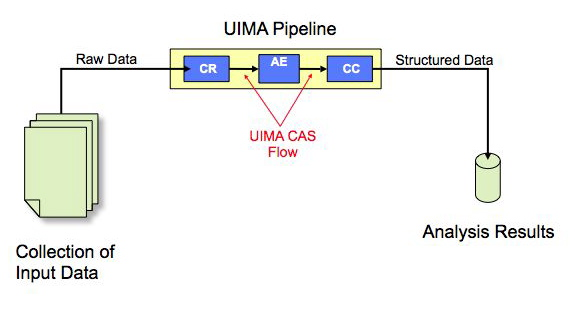
\includegraphics[width=5.5in]{images/uima-pipeline.jpg}
      \caption{Standard UIMA Pipeline}
      \label{fig:UIMA-pipeline}
    \end{figure}

    \paragraph{UIMA-AS  Scaled Pipeline}
    With UIMA-AS the CR is separated into a discrete process and a CAS Multiplier (CM) is introduced 
    into the pipeline as an interface between the CR and the pipeline, as shown in
    \hyperref[fig:UIMA-AS-pipeline]{Figure ~\ref{fig:UIMA-AS-pipeline}} below.
    Multiple pipelines are serviced by the 
    CR and are scaled-out over a computing cluster.  The difficulty with this model is that each
    user is individually responsible for finding and scheduling computing nodes, installing
    communication software such as ActiveMQ, and generally managing the distributed job and
    associated hardware.

    \begin{figure}[H]
      \centering
      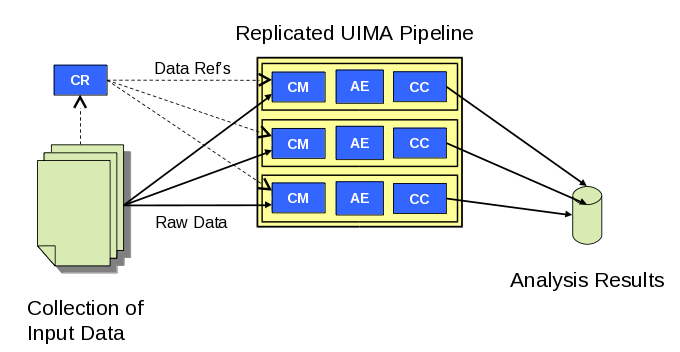
\includegraphics[width=5.5in]{images/uima-as-pipeline.png}
      \caption{UIMA Pipeline As Scaled by UIMA-AS}
      \label{fig:UIMA-AS-pipeline}
    \end{figure}

    \paragraph{UIMA Pipeline Scaled By DUCC}
    DUCC is a UIMA and  UIMA-AS-aware cluster manager.  To scale out work under DUCC the developer
    tells DUCC what the parts of the application are, and DUCC does the work to build the
    scale-out via UIMA/AS, to find and schedule resources, to deploy the parts of the application
    over the cluster, and to manage the jobs while it executes.

    On job submission, the CR is wrapped with a DUCC main class and launched as a Job Driver (or JD).
    The DUCC main class establishes communication with other DUCC components and instantiates the CR.
    If the CR initializes successfully, and indicates that there are greater than 0 work items to process,
    the specified CM, AE and CC components are assembled into an aggregate, wrapped with a DUCC main
    class, and launched as a Job Process (or JP).

	The JP will replicate the aggregate as many times as specified, each aggregate instance running 
	in a single thread. When the aggregate initializes, and whenever an aggregate thread needs work,
	the JP wrapper will fetch the next work item from the JD, as shown in 
    \hyperref[fig:UIMA-AS-pipeline-DUCC]{Figure ~\ref{fig:UIMA-AS-pipeline-DUCC}} below.

    \begin{figure}[H]
      \centering
      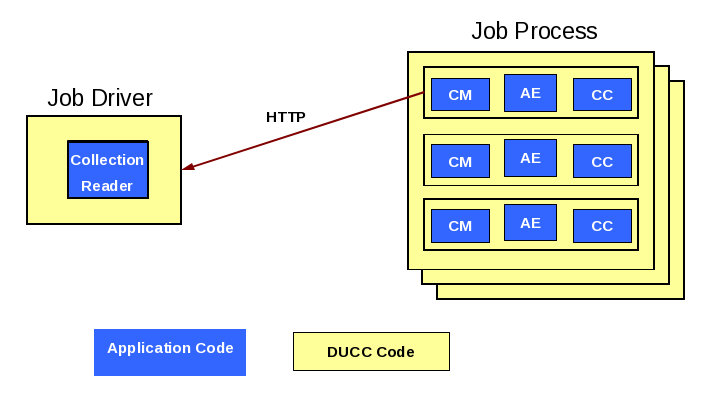
\includegraphics[width=5.5in]{images/ducc-sequential.png}
      \caption{UIMA Pipeline As Automatically Scaled Out By DUCC}
      \label{fig:UIMA-AS-pipeline-DUCC}
    \end{figure}

    \paragraph{UIMA Pipeline with User-Supplied DD Scaled By DUCC}

    Application programmers may supply their own Deployment Descriptors to control intra-process
    threading and scale-out.  If a DD is specified in the job parameters, DUCC will launch each
    JP with the specified UIMA-AS service instantiated in-process,
    as depicted in \hyperref[fig:UIMA-AS-pipeline-DUCC-DD]{Figure ~\ref{fig:UIMA-AS-pipeline-DUCC-DD}} below.
    In this case the user can still specify how many work items to deliver to the service concurrently.

    \begin{figure}[H]
      \centering
      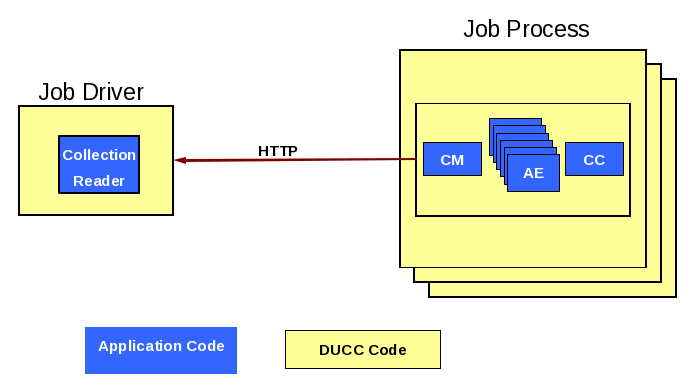
\includegraphics[width=5.5in]{images/ducc-parallel.png}
      \caption{UIMA Pipeline With User-Supplied DD as Automatically Scaled Out By DUCC}
      \label{fig:UIMA-AS-pipeline-DUCC-DD}
    \end{figure}

  
    \section{Error Management }
    DUCC provides a number of facilities to assist error management:
    
    \begin{itemize}
      \item DUCC captures exceptions in the JPs and delivers them
        to the Job Drivers. The JD wrappers implement logic to enforce error thresholds, to identify
        and log errors, and to reflect job problems in the DUCC Web Server.  Error thresholds are
        configurable both globally and on a per-job basis.

      \item Error and timeout thresholds are implemented for both the initialization phase of a pipeline
        and the execution phase.
    
      \item Retry-after-error is supported: if a process has a failure on some CAS after
        initialization is successful, the process is terminated and all affected CASs are retried, up to some
        configurable threshold.

      \item To avoid disrupting existing workloads by a job that will fail to run,
        DUCC ensures that JD and JP processes can successfully initialize before fully scaling out a job.

      \item Various error conditions encountered  while a job is running will prevent a problematic job
        from continuing scale out, and can result in termination of the job.
      \end{itemize}
      
    \section{Cluster and Job Management}
    DUCC supports  management of multiple jobs and multiple users in a distributed cluster:

    \begin{description}
        \item[Multiple User Support] When properly configured, 
          DUCC runs all work under the identity of the submitting user. Logs
          are written with the user's credentials into the user's file space designated at job
          submission.

        \item[Fair-Share Scheduling] DUCC provides a Fair-Share scheduler to equitably share
          resources among multiple users.  The scheduler also supports semi-permanent reservation of machines.

        \item[Service Management] DUCC provides a Service Manager capable of automatically starting, stopping, and
          otherwise managing and querying both UIMA-AS and non-UIMA-AS services in support of jobs.

        \item[Job Lifetime Management and Orchestration] DUCC includes an Orchestrator to manage the
          lifetimes of all entities in the system.

        \item[Node Sharing] DUCC allocates processes for one or more users on a node, each with a specified
          amount of memory.  DUCC's preferred mechanism for constraining memory use is Linux
          Control Groups, or CGroups.  For nodes that do not support CGroups, DUCC agents monitor
          RAM use and kill processes that exceed their share size by a settable fudge factor.

        \item[DUCC Agents] DUCC Agents manage each node's local resources and all
          processes started by DUCC. Each node in a cluster has exactly one Agent. The Agent
          \begin{itemize}
            \item Monitors and reports node capabilities (memory, etc) and performance data (CPU busy,
              swap, etc).
            \item Starts, stops, and monitors all processes on behalf of users.
            \item Patrols the node for ``foreign'' (non-DUCC) processes, reporting them to the
              Web Server, and optionally reaping them.
            \item Ensures job processes do not exceed their declared memory requirements
              through the use of Linux CGroups.
          \end{itemize}

        \item[DUCC Web server] DUCC  provides a web server displaying all aspects of the system:
          \begin{itemize}
              \item All jobs in the system, their current state, resource usage, etc.
                
              \item All reserved resources and associated information (owner, etc.),
                including the ability to request and cancel reservations.
                
              \item All services, including the ability to start, stop, and modify
                service definitions.
                
              \item All nodes in the system and their status, usage, etc. 
                                
              \item The status of all DUCC management processes.  

              \item Access to documentation.
          \end{itemize}


        \item[Cluster Management Support] DUCC provides system management support to:
          \begin{itemize}
              \item Start, stop, and query full DUCC systems.
 
              \item Start, stop, and quiesce individual DUCC components.
 
              \item Add and delete nodes from the DUCC system.
 
              \item Discover DUCC processes (e.g. after partial failures).
 
              \item Find and kill errant job processes belonging to individual users.
                
              \item Monitor and display inter-DUCC messages.
          \end{itemize}
      \end{description}

    
    \section{Security Measures}
    The following DUCC security measures are provided:

    \begin{description}
    \item[user credentials] DUCC instantiates user processes using a setuid root executable named ducc\_ling.
    See more at \hyperref[sec:duccling.security]{\em ducc\_ling}.
    \item[command line interface] The CLI employs HTTP to send requests
    to the DUCC controller.  The CLI creates and employs public and private
    security keys in the user's home directory for authentication of HTTP
    requests.  The controller validates requests via these same security keys.
    \item[webserver] The webserver facilitates operational control and
    therefore authentication is desirable. 
    \begin{itemize}
    \item[\textit{user}] Each user has the ability to control certain aspects of
    only his/her active submissions.
    \item[\textit{admin}] Each administrator has the ability to control certain
    aspects of any user's active submissions, as well as modification of some
    DUCC operational characteristics.
    \end{itemize}
    A simple interface is provided so
    that an installation can plug-in a site specific authentication mechanism
    comprising userid and password.
    \item[ActiveMQ] DUCC uses ActiveMQ for administrative communication.
    AMQ authentication is used to prevent arbitrary processes from participating.
    But when testing DUCC on a simulated cluster the AMQ broker runs without any access restrictions 
    so that it can be used as an application broker for UIMA-AS services used in simulation tests. 
    See \hyperref[subsec:sim.start-sim]{{\em start\_sim}}.
    \end{description}
    
    \subsection{ducc\_ling}   
    \label{sec:duccling.security}
           ducc\_ling contains the following functions, which the security-conscious may verify by examining
       the source in \duccruntime/duccling.  All sensitive operations are performed only AFTER switching
       userids, to prevent unauthorized root access to the system.
       \begin{itemize}
         \item Changes it's real and effective userid to that of the user invoking the job.
         \item Optionally redirects its stdout and stderr to the DUCC log for the current job.
         \item Optionally redirects its stdio to a port set by the CLI, when a job is submitted.
         \item ``Nice''s itself to a ``worse'' priority than the default, to reduce the chances
           that a runaway DUCC job could monopolize a system.
         \item Optionally sets user limits.
         \item Prints the effective limits for a job to both the user's log, and the DUCC agent's log.
         \item Changes to the user's working directory, as specified by the job.
         \item Optionally establishes LD\_LIBRARY\_PATH 
           for the job from the environment variable  {\tt DUCC\_LD\_LIBRARY\_PATH}
           if set in the DUCC job specification. (Secure Linux systems will
           prevent LD\_LIBRARY\_PATH 
           from being set by a program with root authority, so this is
           done AFTER changing userids).
         \item  ONLY user {\em ducc} may use the ducc\_ling program in
           a privileged way. Ducc\_ling contains checks to prevent even user {\em root} from using it for
           privileged operations. 

       \end{itemize}
    
    
    \section{Security Issues}
    The following DUCC security issues should be considered:
    
    \begin{description}
    \item[submit transmission 'sniffed'] In the event that the DUCC submit
    command is 'sniffed' then the user authentication mechanism is compromised
    and user masquerading is possible.  That is, the userid encryption mechanism
    can be exploited such that user A can submit a job pretending to be user B.
    \item[user \textit{ducc} password compromised] In the event that the \textit{ducc}
    user password is compromised then the root privileged command
    \textbf{ducc\_ling} can be used to become any other user except root.
    \item[user \textit{root} password compromised] In the event that the
    \textit{root} user password is compromised DUCC provides no protection. 
    That is, compromising the root user is equivalent to compromising the DUCC
    user password.
    \end{description}  
     
